%%%%%%%%%%%%%%%%%%%%%%%%%%%%%%%%%%%%%%%%%%%%%%%%%%%%%%%%%%%%%%
%% Carlos Segarra's Beamer Presentation Template. All credits
%% to Vincent Labatut from whom I took the template and added
%% my own flavour to it. Kudos to <vincent.labatut@univ-avignon.fr>
%%%%%%%%%%%%%%%%%%%%%%%%%%%%%%%%%%%%%%%%%%%%%%%%%%%%%%%%%%%%%%
% setup Beamer
\documentclass[10pt,    % default is 11pt, use 10pt for more compact slides
%    handout,            % collapse all overlays (=animations) and video-invert console text
    english,            % presentation language (theme supports only french & english)
    xcolor=table,       % colors in the tables
    envcountsect,        % include section number in theorem numbers
    aspectratio=169     % Using 16:9 aspect ratio because 2019
]{beamer}

%%%%%%%%%%%%%%%%%%%%%%%%%%%%%%%%%%%%%%%%%%%%%%%%%%%%%%%%%%%%%%
% setup the theme
%\usepackage{au/sty/beamerthemeAU}         % no option at all
\usepackage[light]{csg-temp/sty/beamerthemeAU}   % the "light" option only changes the title and section pages

%%%%%%%%%%%%%%%%%%%%%%%%%%%%%%%%%%%%%%%%%%%%%%%%%%%%%%%%%%%%%%
% setup side notes
\usepackage{pgfpages}                                   % comment all 3 below lines to hide notes
%\setbeameroption{show notes}                           % alternate content and note slides
%\setbeameroption{show only notes}                      % only note slides
%\setbeameroption{show notes on second screen=right}    % dualscreen: right, left, top, bottom
%\usepackage{enumitem}

%%%%%%%%%%%%%%%%%%%%%%%%%%%%%%%%%%%%%%%%%%%%%%%%%%%%%%%%%%%%%%
% name of the biblatex file
\addbibresource{biblio.bib}

%%%%%%%%%%%%%%%%%%%%%%%%%%%%%%%%%%%%%%%%%%%%%%%%%%%%%%%%%%%%%%
% External Packages
\usepackage{datenumber}
\usepackage{varwidth}

%%%%%%%%%%%%%%%%%%%%%%%%%%%%%%%%%%%%%%%%%%%%%%%%%%%%%%%%%%%%%%
% Name Definitions via commands
\newcommand{\projName}{\textsc{MedSpark}\xspace}
\newcommand*\blackcircled[1]{\tikz[baseline=(char.base)]{
            \node[shape=circle,fill=fgRed,inner sep=0.5pt] (char) {\textcolor{white}{#1}};}}

%%%%%%%%%%%%%%%%%%%%%%%%%%%%%%%%%%%%%%%%%%%%%%%%%%%%%%%%%%%%%%
% title and subtitle of the presentation (the latter is optional)
\subtitle{CFIS-UPC Joint Bachelor's Thesis Defense} % leave empty if no subtitle
\title[TEEs for Secure Stream Processing] % leave empty for no title in footer
    {\normalsize CFIS-UPC Joint Bachelor's Thesis Defense \\ \Large Using Trusted Execution Environments for Secure Stream Processing of Medical Data}
\subtitle{\small \textmd{In partial fulfillment of the requirements for the} \\
\normalsize Bachelor's Degree in Mathematics \\ \small \textmd{and} \\ \normalsize Bachelor's Degree in Telecommunications Technologies and Services Engineering \vspace{-10pt}} % leave empty if no subtitle
%%%%%%%%%%%%%%%%%%%%%%%%%%%%%%%%%%%%%%%%%%%%%%%%%%%%%%%%%%%%%%
% date of the presentation (leave empty for no date, default is today)
\date[Thursday, May 30th] % leave empty for no date in footer
    {\datedayname, \today}
%%%%%%%%%%%%%%%%%%%%%%%%%%%%%%%%%%%%%%%%%%%%%%%%%%%%%%%%%%%%%%
% authors and their affiliations (the latter is optional)
\author[] % leave empty for no author in footer
{\textit{Author:} C.~Segarra\inst{1, 2} \hfill \textit{Supervisors:} R.~Delgado-Gonzalo\inst{1}, J.A.~Rodr\'iguez\inst{2}}
\institute[] % (short affiliation not used in this theme)
{\inst{1} Swiss Center for Electronics and Microtechnology (CSEM), Switzerland, \texttt{\{first.last\}@csem.ch} \and
\inst{2} Universitat Polit\`ecnica de Catalunya (UPC), Spain, \texttt{\{carlos.segarra@estudiant., jose.fonollosa@\}upc.edu}
}
%{\inst{1} Computer Science Lab, Avignon University -- LIA EA 4128 \texttt{\{firstname.lastname\}@univ-avignon.fr}
%\and \inst{2} Institute of Disruptive Innovation, University of Excellence \texttt{\{firstname.lastname\}@univ-excell.fr}
%}
%%%%%%%%%%%%%%%%%%%%%%%%%%%%%%%%%%%%%%%%%%%%%%%%%%%%%%%%%%%%%%
% optional: additional logo (ex. lab)
\titlegraphic{
\includegraphics[width=3cm,]{images/logo-csem.png}}
% if you want several logos, put them in a box
%\titlegraphic{\parbox{3cm}{
\includegraphics[width=3cm,]{images/ceri_logo.pdf}\newline
\includegraphics[width=3cm,]{images/lia_logo.pdf}}}
%%%%%%%%%%%%%%%%%%%%%%%%%%%%%%%%%%%%%%%%%%%%%%%%%%%%%%%%%%%%%%

%%%%%%%%%%%%%%%%%%%%%%%%%%%%%%%%%%%%%%%%%%%%%%%%%%%%%%%%%%%%%
% Presentation speciphic packages
% \usepackage{multicol}
% \usepackage[titles]{tocloft}
% \renewcommand{\cftchapfont}{\normalfont\bfseries}
\usetikzlibrary{decorations.pathmorphing, patterns}
\usepackage{tabularx}
\newcolumntype{L}[1]{>{\raggedright\arraybackslash}p{#1}}
\newcolumntype{C}[1]{>{\centering\arraybackslash}p{#1}}
\newcolumntype{R}[1]{>{\raggedleft\arraybackslash}p{#1}}
%%%%%%%%%%%%%%%%%%%%%%%%%%%%%%%%%%%%%%%%%%%%%%%%%%%%%%%%%%%%%

%%%%%%%%%%%%%%%%%%%%%%%%%%%%%%%%%%%%%%%%%%%%%%%%%%%%%%%%%%%%%%
\begin{document}
%%% title page
\begin{frame}
  \titlepage
\end{frame}

%%% outline of the presentation
\begin{frame}{Session Outline}
    \begin{columns}[T,onlytextwidth]
        \hspace{1.25cm}
        \begin{column}{.4\textwidth}
            \tableofcontents[sections={1-2}]
    %        [hideallsubsections] % un-comment this line to hide sub-sections
        \end{column}
        \hspace*{-3.25cm}
        \begin{column}{.4\textwidth}
            \tableofcontents[sections={3-5}]
    %        [hideallsubsections] % un-comment this line to hide sub-sections
        \end{column}
    \end{columns}
\end{frame}

\section{Introduction}
\label{sec:introduction}
\sectionframe

\subsection{Project Generalities}

\begin{frame}
    \frametitle{Introduction}
    \framesubtitle{Project Generalities and Collaborators}

    \vspace{-10pt}

    \begin{itemize}
        \item \textbf{Bachelor Thesis} whilst an intern @ \textbf{Swiss Center for Electronics and Microtechnology (CSEM)} - Sup. R.~Delgado-Gonzalo
        \item Work on \textbf{\textcolor{fgRed}{privacy-preserving}} data processing \textrightarrow \textbf{Trusted Hardware}
        \item Two accepted publications: \textbf{EMBC '19} $[1]$ and \textbf{DAIS '19} $[2]$ 
        \item Joint work with:
        \begin{itemize}
            \item \textbf{CSEM} - Ricard Delgado-Gonzalo and Enric Muntan\'e
            \item \textbf{Universit\'e de Neuch\^atel} - Valerio Schiavoni
            \item \textbf{Imperial College London} - Pierre-Louis Aublin and Peter Pietzuch
        \end{itemize}
    \end{itemize}

    \vspace{5pt}

    \begin{columns}[b]
        \centering
        \begin{column}{.2\textwidth}
            
\includegraphics[width=2.5cm]{images/unine-no-bg-no-letter.png}
        \end{column}
        \begin{column}{.2\textwidth}
            \hspace*{-30pt}
\includegraphics[width=4cm]{images/logo-csem.png}
        \end{column}
        \begin{column}{.2\textwidth}
            
\includegraphics[width=3cm]{images/imperial-college.png}
        \end{column}
    \end{columns}

    \vspace{10pt}

    \tiny
    \begin{description}
        \item $[1]$ C.~Segarra, E.~Muntané, M.~Lemay, V.~Schiavoni, R.~Delgado-Gonzalo, \textit{\textbf{"Secure Stream Processing for Medical Data"}}, IEEE EMBC'19, Berlin, Germany, July 23-27, 2019.
        \item $[2]$ C.~Segarra, M.~Lemay, R.~Delgado-Gonzalo, P.-L.~Aublin, P.~Pietzuch, V.~Schiavoni, \textbf{\textit{"Using Trusted Execution Environments for Secure Stream Processing of Medical Data"}}, DAIS'19, Copenhagen, Denmark, June 17-21, 2019.
    \end{description}

\end{frame}

\subsection{Motivation}

\begin{frame}
    \frametitle{Motivation}
    \framesubtitle{Why do we need secure big data processing engines?}

    \vspace{-20pt}

    \begin{figure}[H]
        \centering
        \resizebox{0.9\linewidth}{!}{\begin{tikzpicture}
    % Colors definition: latexcolor.com
    \definecolor{blue0}{RGB}{0,25,51}
    \definecolor{blue1}{RGB}{0,51,102}
    \definecolor{blue2}{RGB}{0,128,255}
    \definecolor{blue3}{RGB}{153,204,255}
    \definecolor{yellow}{RGB}{250,165,25}
    \definecolor{lightyellow}{RGB}{229,208,66}
    \definecolor{ashgrey}{rgb}{0.7, 0.75, 0.71}
    \definecolor{x11gray}{rgb}{0.75, 0.75, 0.75}

    %% Nodes
    % We want to
    \node[align=center] (first) at (0,0) {\textbf{We want to:}};
    \node[below of=first, align=center, yshift=10pt] (second) {\textbf{Process} large amounts of \textbf{\textcolor{fgRed}{sensitive}} information};
    % Outsourcing
    \node[below of=second, align=center, visible on=<2->] (third) {\textbf{\textcolor{fgRed}{Outsourcing}} of data \textbf{storage} and \textbf{processing}};
    % Cloud Provider 
    \node[below of=third, align=center, visible on=<3->] (fourth) {Cloud tenant \textbf{\textcolor{fgRed}{can}} access \textbf{protected} data};
    % This is...
    \node[below of=fourth, align=center, visible on=<4->] (fifth) {\textbf{\textcolor{red}{UNACCEPTABLE FOR INDUSTRIES IN THE MEDICAL DOMAIN}}};

    %% Arrows
    \draw[->, very thick, blue2!50!blue1, visible on=<2->] (second) -- (third) node[pos=.5, align=left, anchor=west, xshift=8pt] {\textcolor{blue2!50!blue1}{Generally requires...}};
    \draw[->, very thick, blue2!50!blue1, visible on=<3->] (third) -- (fourth) node[pos=.5, align=left, anchor=west, xshift=8pt] {\textcolor{blue2!50!blue1}{Generally means...}};
    \draw[->, very thick, blue2!50!blue1, visible on=<4->] (fourth) -- (fifth) node[pos=.5, align=left, anchor=west, xshift=8pt] {\textcolor{blue2!50!blue1}{This is...}};
\end{tikzpicture}
}
    \end{figure}

\end{frame}

\section{Background}
\label{sec:background}
\sectionframe

\subsection{Technical Background}

\begin{frame}
    \frametitle{Trusted Execution Environments (TEE)}
    \framesubtitle{Formal definition, examples and availability}

    \begin{exampleblock}{Trusted Execution Environment}
        A \textbf{TEE} is a secure area of a main processor. It guarantees code and data loaded inside to be protected with respect to \textbf{\textcolor{fgRed}{confidentiality}} and \textbf{\textcolor{fgRed}{integrity}}. 
    \end{exampleblock}

    \only<2>{
    \begin{itemize}
        \item Available on a variety of commodity CPUs. Namely:
    \end{itemize}
    }

    % TODO: missing Intel SGX and Arm Trustzone logo
    \visible<3>{
    \begin{columns}
        \begin{column}{.45\textwidth}
            \begin{figure}[h!]
                \centering
                \includegraphics[width=2.2cm]{images/intel-sgx-enclave.jpg}
                \caption*{\textbf{Intel SGX} Available on consumer-grade CPUs starting from architecture codename \textit{Skylake}.}
            \end{figure}
        \end{column}
        \begin{column}{.45\textwidth}
            \begin{figure}[h!]
                \centering
                
\includegraphics[width=3cm]{images/Arm-TrustZone-Logo.png}
                \caption*{\textbf{Arm Trustzone} Available on Cortex-A processors and v8 Cortex-M23 and Cortex-M33.}
            \end{figure}
        \end{column}
    \end{columns}
    }

\end{frame}

\begin{frame}
    \frametitle{Intel Software Guard eXtensions}
    \framesubtitle{Definition, Threat Model and Known Vulnerabilities}

    \begin{columns}
        \begin{column}{0.45\textwidth}
            \only<1>{
                \vspace{-35pt}
                \begin{itemize}
                    \setlength\itemsep{5pt}
                    \item \textbf{Intel Software Guard eXtensions (SGX)} are a set of instructions and memory access extensions that enable applications to create \textbf{hardware-protected areas} in their address space called \textbf{\textcolor{fgRed}{enclaves}}. 
                    \item Security perimiter includes \textbf{\textcolor{fgRed}{only}} the internals of the CPU package.
                    % \item Traffic between CPU and main memory is kept \textbf{confidential} by the \textbf{\textcolor{fgRed}{MEE}}.
                    \item An \textbf{\textcolor{fgRed}{attestation protocol}} verifies that code is running in a \textbf{genuine enclave} and that it has not been tampered.
                \end{itemize}
            }
%            \only<2>{
%                \vspace{-35pt}
%                \begin{itemize}
%                    \setlength\itemsep{8pt}
%                    \item Threat model assumes an adversary with access to \textbf{\textcolor{fgRed}{privileged software}}. Such as: VMM, BIOS, OS, ...
%                    \item Limited \textbf{\textcolor{fgRed}{enclave memory}}, costly entry/exit and expensive \textbf{\textcolor{fgRed}{paging}}.
%                    \item \textbf{Traffic Analysis}, \textbf{Side-Channel} and \textbf{Speculative Execution} attacks have been succesful. Most \textbf{\textcolor{fgRed}{patched}} as of today.
%                \end{itemize}
%            }
        \end{column}
        \begin{column}{0.5\textwidth}
            \visible<1->{
                    \begin{figure}[H]
                    \centering
                    \resizebox{0.9\linewidth}{!}{\resizebox{\linewidth}{!}{
\begin{tikzpicture}

    % Main outline
    %\draw[fill=green1] (0,0) rectangle (10, 1) node[pos=.5] {Privileged System Code, OS, VMM};
    \draw[fill=gray!10] (0, 0) rectangle (10, 8.5);

    % Unsecure Part
    \node[align=center] at (2.25, 7.5) {\textbf{Untrusted Code}};
    \draw[dashed, fill=white] (0.5, 0.5) rectangle (4, 7.0);
    \node at (1.25, 1.25) {
\includegraphics[width=25pt]{img/hacker.png}};
    \draw[->,thick, decorate,decoration={snake, post=lineto, post length=1mm}] (2.25, 6.5) -- (2.25, 5.75) node[pos=.3,anchor=west] {\blackcircled{1}};
    \node[align=center] at (2.25, 5.5) {\texttt{Create Enclave}};
    \draw[->,thick, decorate,decoration={snake, post=lineto, post length=1mm}] (2.25, 5) -- (2.25, 4) node[pos=.5,anchor=west] {\blackcircled{2}};
    \node[align=center] at (2.25, 3.5) {\texttt{Call Trusted} \\ \texttt{Function}};
    \draw[->,thick, decorate,decoration={snake, post=lineto, post length=1mm}] (2.25, 3) -- (2.25, 2) node[pos=.3,anchor=west] {\blackcircled{7}};
    \draw[->, very thick] (4, 5.25) -- (5.5, 5.25) node[pos=.5,anchor=south] {\blackcircled{3}};

    % Secure Part
    \node[align=center] at (7.75, 7.5) {\textbf{Trusted Code}};
    \draw[fill=white,pattern=north west lines,pattern color=gray!50] (6, 0.5) rectangle (9.5, 7.0);
    \node at (8.75, 1.25) {
\includegraphics[width=25pt]{img/intel-sgx.png}};
    \node[align=center] at (5.55, 6.5) {\small{Call} \\ \small{Gate}};
    \draw[fill=gray!80] (5.5, 5.5) rectangle (6, 6.0);
    \draw[fill=gray!80] (5.5, 5.0) rectangle (6, 5.5);
    \draw[fill=gray!80] (5.5, 4.5) rectangle (6, 5.0);
    \draw[rounded corners, dashed, fill=white] (6.5, 2.5) rectangle (9, 5.75);
    \draw[->, very thick] (5.75, 5.25) -- (6.75, 5.25) node[pos=.5,anchor=south] {\blackcircled{4}};
    \node[align=center] at (7.75, 5.25) {\texttt{Execute}};
    \draw[->,thick, decorate,decoration={snake, post=lineto, post length=4mm}] (7.75, 5) -- (7.75, 3.25) node[pos=.5,anchor=west] {\blackcircled{5}};
    \node[align=center] at (7.75, 3) {\texttt{Return}};
    \draw[->, very thick] (6.75, 3) -- (4, 3) node[pos=.6, anchor=south] {\blackcircled{6}};
\end{tikzpicture}}
}
                    \caption{Intel SGX Operating Principles.}
                    \label{fig:sgx-principles}
                \end{figure}
            }
        \end{column}
    \end{columns}
\end{frame}

\begin{frame}
    \frametitle{SGX-Spark}
    \framesubtitle{Running Spark Jobs inside Enclaves}


    \begin{columns}
        \begin{column}{0.65\textwidth}
            \only<1>{
                \vspace{-35pt}

                \textbf{\textcolor{fgRed}{SGX-Spark}}

                \begin{itemize}
                    %\setlength\itemsep{13pt}
                    \item Based on Apache Spark, SGX-Spark is a framework under-development at the \textbf{Imperial College London} (co-authors) to enable seamless deployment of \textbf{Spark} jobs inside \textbf{enclaves}.
                    \item Protect \textbf{confidentiality} and \textbf{integrity} of existing Spark jobs \textbf{\textcolor{fgRed}{without}} modifications to the application code.
                    \item Execute only \textbf{sensitive} parts of the application \textbf{\textcolor{fgRed}{inside}} the enclave. Leave information outside the enclave \textbf{encrypted}.
                \end{itemize}
            }
        \end{column}
        \begin{column}{0.3\textwidth}
            \visible<1->{
                \begin{figure}[H]
                    \centering
                    \resizebox{0.9\linewidth}{!}{\resizebox{.4\textwidth}{!}{
\begin{tikzpicture}
    % Colors definition: latexcolor.com
    \definecolor{ashgrey}{rgb}{0.7, 0.75, 0.71}
    \definecolor{x11gray}{rgb}{0.75, 0.75, 0.75}

    
    % Main outline
    \draw[fill=gray!10] (0,0) rectangle (3, 4);

    % First Layer
    % Shared Memory
    \draw[fill=white] (0.25, 0.25) rectangle (2.75, 0.5) node[pos=.5] {\tiny SHM};
    \node at (0.45, 0.375) {
\includegraphics[width=5pt]{img/hacker.png}};

%    \draw[fill=white] (0.25, 0.25) rectangle (1.45, 0.825) node[pos=.5] {\tiny{OS}};;
%    \node at (0.45, 0.45) {
\includegraphics[width=8pt]{img/hacker.png}};
%    \draw[fill=white, pattern=north west lines,pattern color=gray!50] (1.55, 0.25) rectangle (2.75, 0.825) node[pos=.5] {\tiny{SGX}};
%    \node at (2.55, 0.45) {
\includegraphics[width=8pt]{img/intel-sgx.png}};

    % Second Layer
    \draw[fill=white] (0.25, 0.6) rectangle (1.45, 1.55) node[pos=.5, xshift=2pt, yshift=3pt, align=center] {\tiny{Spark} \\[-9pt] \tiny{Worker}};
    \node at (0.45, 0.8) {
\includegraphics[width=8pt]{img/hacker.png}};
    \draw[fill=white, pattern=north west lines,pattern color=gray!50] (1.55, 0.6) rectangle (2.75, 1.55) node[pos=.5, xshift=-3pt, yshift=3pt, align=center] {\tiny{Worker} \\[-9pt] \tiny{Enclave}};
    \node at (2.55, 0.8) {
\includegraphics[width=8pt]{img/intel-sgx.png}};

    % Third Layer
    \draw[fill=white] (0.25, 1.65) rectangle (1.45, 3.4);
    \node[align=center] at (0.85, 2.65) {\tiny{Driver} \\[-10pt] \tiny{\&} \\[-10pt] \tiny{App Entry} \\[-10pt] \tiny{Point}};
    \node at (0.45, 1.85) {
\includegraphics[width=8pt]{img/hacker.png}};
    \draw[fill=white, pattern=north west lines,pattern color=gray!50] (1.55, 1.65) rectangle (2.75, 3.4);
    \node[align=center] at (2.15, 2.85) {\tiny{Driver} \\[-10pt] \tiny{Enclave}};
    \node at (2.55, 1.85) {
\includegraphics[width=8pt]{img/intel-sgx.png}};
    % Spark Tasks
    \draw[fill=white] (1.6, 2.1) rectangle (1.95, 2.4) node[pos=.5] {\tiny{T$1$}}; 
    \node at (2.15, 2.25) {\tiny{$\cdots$}};
    \draw[fill=white] (2.35, 2.1) rectangle (2.7, 2.4) node[pos=.5] {\tiny{T$N$}}; 

    % Spark Master
    \draw[fill=white] (0.25, 3.5) rectangle (2.75, 3.75) node[pos=.5] {\tiny{Spark Master}};
    \node at (0.45, 3.625) {
\includegraphics[width=5pt]{img/hacker.png}};

\end{tikzpicture}}
}
                    \caption{SGX-Spark Collaborative Structure.}
                    \label{fig:sgx-spark}
                \end{figure}
            }
        \end{column}
    \end{columns}
\end{frame}

\subsection{Medical Background}

\begin{frame}
    \frametitle{Medical Background}
    \framesubtitle{Cardiac Monitoring, ECG, PPG, and HRV}

    \only<1>{
        
        \vspace{10pt}

        \begin{itemize}
            \item Our solution is \textbf{\textcolor{fgRed}{independent of the chosen data streams}}, hence it could be leveraged in a variety of domains where privacy might be a concern. However, 
            \item The data streams used for this project belong to the \textbf{medical} domain, in particular, they are obtained from human \textbf{\textcolor{fgRed}{cardiac activity monitoring}}. The two most standard procedures are:
            \begin{enumerate}
                \item \textbf{ECG:} measure heart's electrical activity over time. \textit{E.g:} chest straps.-%\textrightarrow Chest-based sensors
                \item \textbf{PPG:} measure blood's volume variation over time. \textit{E.g:} smartwatches and pulse oximeters.
            \end{enumerate}
        \end{itemize}
    }

    \begin{itemize}
        \item Either if the data comes from an \textbf{ECG} or \textbf{PPG} based sensor, we are interested in the \textbf{\textcolor{fgRed}{inter-beat intervals}} from the generated diagram ($23 - 69$ B per second per user).
        \item From an \textbf{ECG} we can obtain obtain these intervals from the time between \textbf{\textcolor{fgRed}{R peaks}}, abbreviated as RR intervals (Figure \ref{fig:ecg-hrv}).
        \item With their \textbf{timestamps} we compute a live analysis of the \textbf{\textcolor{fgRed}{Heart Rate Variability (HRV)}}.
    \end{itemize}
    \visible<2->{
        \begin{figure}[H]
            \centering
            \resizebox{0.75\linewidth}{!}{\resizebox{\linewidth}{!}{
\begin{tikzpicture}
    % Colors definition
    \pgfdeclaredecoration{single pulse}{initial}{
    \state{initial}[width=\pgfdecoratedinputsegmentlength]
    {%
        % Initial Line
        \pgfpathlineto{\pgfpoint{0.1*\pgfdecoratedinputsegmentlength}{0mm}}%    
        % P Peak
        \pgfpathsine{\pgfpoint{0.2\pgfdecorationsegmentlength}{0.15\pgfdecorationsegmentamplitude}}%
        \pgfpathcosine{\pgfpoint{0.2\pgfdecorationsegmentlength}{-0.15\pgfdecorationsegmentamplitude}}%
        % P - Q Line
        \pgfpathlineto{\pgfpoint{0.6\pgfdecorationsegmentamplitude}{0mm}}%
        % Q Valley
        \pgfpathsine{\pgfpoint{0.1\pgfdecorationsegmentlength}{-0.15\pgfdecorationsegmentamplitude}}
        \pgfpathcosine{\pgfpoint{0.01\pgfdecorationsegmentlength}{0.15\pgfdecorationsegmentamplitude}}%
        % R Peak
        \pgfpathsine{\pgfpoint{0.15\pgfdecorationsegmentlength}{\pgfdecorationsegmentamplitude}}%
        \pgfpathcosine{\pgfpoint{0.15\pgfdecorationsegmentlength}{-\pgfdecorationsegmentamplitude}}%
        % S Valley
        \pgfpathsine{\pgfpoint{0.15\pgfdecorationsegmentlength}{-0.5\pgfdecorationsegmentamplitude}}
        \pgfpathcosine{\pgfpoint{0.15\pgfdecorationsegmentlength}{0.5\pgfdecorationsegmentamplitude}}%
        % S to T line
        \pgfpathlineto{\pgfpoint{1.25\pgfdecorationsegmentamplitude}{0mm}}%
        % T Peak
        \pgfpathsine{\pgfpoint{0.8\pgfdecorationsegmentlength}{0.3\pgfdecorationsegmentamplitude}}%
        \pgfpathcosine{\pgfpoint{0.8\pgfdecorationsegmentlength}{-0.3\pgfdecorationsegmentamplitude}}%
        % Last Line
        \pgfpathlineto{\pgfpointdecoratedinputsegmentlast}%
    }
    \state{final}{}%
    }

    \fill[gray!10, draw=black] (-0.75, -0.75) rectangle (6.25, 1.75);
    \node at (-0.5, -0.5) {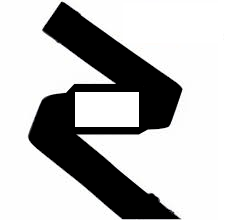
\includegraphics[width=10pt]{img/hrband.png}};
    %\node at (5.5, 1.5) {\textbf{\small{Sensor}}};

    \draw[->, dashed] (5.55,0) -- (6,0) node[pos=.5, anchor=north, xshift=-10pt] {\tiny{Time ($s$)}};
    \draw[->, dashed] (0,0) -- (0,1.25) node[anchor=south, xshift=10pt] {\tiny{Amplitude ($mV$)}};
    \draw[decoration={single pulse,amplitude=8mm,segment length=2mm},decorate] (0,0) -- (2,0);
    \draw[decoration={single pulse,amplitude=8mm,segment length=2mm},decorate] (2,0) -- (4,0);
    \draw[decoration={single pulse,amplitude=6mm,segment length=2mm},decorate] (4,0) -- (5.5,0);
    \draw[<->, dashed, thick] (0.55, 0.7) -- (2.5, 0.7);
    \draw[<->, dashed, thick] (2.55, 0.55) -- (4.35, 0.55);
    \node[align=center] at (0.5, 0.95) {\tiny{$\text{R}_0$}};
%    \node[align=center] at (2.2, 0.3) {\tiny{$\text{P}_1$}};
%    \node[align=center] at (2.45, -0.2) {\tiny{$\text{Q}_1$}};
%    \node[align=center] at (2.7, -0.55) {\tiny{$\text{S}_1$}};
%    \node[align=center] at (3.15, 0.38) {\tiny{$\text{T}_1$}};
    \node[align=center] at (2.5, 0.95) {\tiny{$\text{R}_1$}};
    \node[align=center] at (4.25, 0.8) {\tiny{$\text{R}_2$}};

    % Signal
    \fill[black] (6.5, 0) circle (0.05);
    \draw (6.75, -0.15) arc (-20:20:0.5);
    \draw (6.95, -0.25) arc (-30:30:0.5);
    \draw (7.15, -0.35) arc (-40:40:0.5);

    % Data file
    \node[align=center] at (9, 1.2) {\tiny{\textbf{\texttt{gateway://data/data\_file.csv}}}};
    \draw (7.45, -0.75) -- (7.45, 1) -- (10.5,1) -- (10.5, -0.5) to[out=180, in=0] (7.45, -0.75);
    \node[align=center] at (9, 0.2) {\tiny{\texttt{t}$\left(\text{R}_1\right)$, \xspace\texttt{t}$\left(\text{R}_1\right)$ - \texttt{t}$\left(\text{R}_0\right)$} \\ \tiny{\texttt{t}$\left(\text{R}_2\right)$, \xspace\texttt{t}$\left(\text{R}_2\right)$ - \texttt{t}$\left(\text{R}_1\right)$} \\ \tiny{\textbf{$\vdots$}}};
\end{tikzpicture}}
}
            \caption{Schematic representation of an ECG signal and the data we gather.\label{fig:ecg-hrv}}
        \end{figure}
    }

\end{frame}

\section{Secure Stream Processing of Medical Data}
\label{sec:medspark}
\sectionframe

\subsection{Project Goals \& Envisioned Use Case}

\begin{frame}
    \frametitle{Secure Stream Processing of Medical Data}
    \framesubtitle{Project Goals \& Envisioned Scenario}

    \only<1>{
        
        \vspace{10pt}

        \begin{itemize}
            \item \textbf{\textcolor{fgRed}{Goal:}} use SGX-Spark to implement a streaming platform that gathers data from sensors and securely outsources computation.
            \begin{itemize}
                \item Deploy in an existing medical environment.
                \item Perform stress tests to assess the system's robustness and reliability.
                \item Evaluate and quantify the overhead of providing strong security guarantees.
            \end{itemize}
        \end{itemize}
    }

    The \textbf{chosen scenario} involves:
    \begin{enumerate}
        \item ECG data streamed from a \textbf{sensor} to a \textbf{gateway}
        \item Real-time processing with \textbf{HRV} algorithms: SDNN and HRV Bands analysis.
        \begin{itemize}
            \item \textbf{SDNN:} rolling standard deviation of NN (RR) intervals.
            \item \textbf{HRV Bands:} rolling DFT and LF/HF component measure.
        \end{itemize}
        \item Suport for \textbf{storage} and result \textbf{post-processing}
    \end{enumerate}

    \visible<2->{
        \begin{figure}[H]
            \centering
            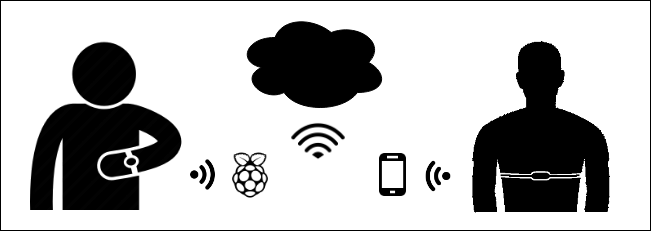
\includegraphics[width=.5\linewidth]{images/wearable-ecosystem.png}
            \caption{Wearable-enabled ecosystem of our platform.}
        \end{figure}
    }

\end{frame}

\subsection{Architecture \& Implementation}

\begin{frame}
    \frametitle{System Architecture}
    \framesubtitle{Component Analysis and Execution Workflow}

    \begin{figure}[H]
        \centering
        \resizebox{0.9\linewidth}{!}{\resizebox{\linewidth}{!}{
\begin{tikzpicture}
    % Colors definition: latexcolor.com
    \definecolor{ashgrey}{rgb}{0.7, 0.75, 0.71}
    \definecolor{x11gray}{rgb}{0.75, 0.75, 0.75}
    \definecolor{metal}{rgb}{0.43, 0.5, 0.5}

    
    % Main outline
    % Background
    \draw[fill=gray!10] (0, 2.75) rectangle (6.75, 6.0);

    % Client Side
    % Client boxes line
    % Client 1
    \draw[fill=gray!5] (0,1.5) rectangle (2, 2.25);
    \node at (1.6, 1.825) {
\includegraphics[width=10pt]{img/smartwatch.png}};
    \node at (1.05, 1.825) {
\includegraphics[width=10pt]{img/wifi-signal.png}};
    \node at (0.4, 1.825) {
\includegraphics[width=15pt]{img/raspberry.png}};
    % Client 2
    \draw[fill=gray!5] (2.5,1.5) rectangle (4.5, 2.25);
    \node at (2.9, 1.825) {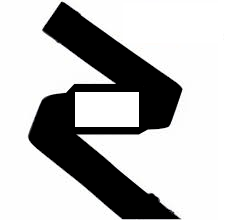
\includegraphics[width=10pt]{img/hrband.png}};
    \node at (3.5, 1.825) {
\includegraphics[width=10pt]{img/wifi-right.png}};
    \node at (4.1, 1.825) {
\includegraphics[width=15pt]{img/raspberry.png}};
    % Client 3
    \node at (5.265, 1.85) {$\cdots$};
    \draw[fill=gray!5] (5.85,1.5) rectangle (6.9, 2.25) node[pos=.5] {\tiny{Client $m$}};
    \draw[fill=gray!5] (8.875,1.5) rectangle (9.625, 2.25) node[pos=.5] {\tiny{Client}};
    % Lines to filesystem
    \draw[<->, dashed, thick] (0.4, 2.25) -- (0.4, 3.5) -- (1, 3.5);
    \draw[<->, dashed, thick] (4.1, 2.25) -- (4.1, 2.35) -- (1.35, 2.35) -- (1.35, 3);
    \draw[<->, dashed, thick] (6.3725, 2.25) -- (6.3725, 2.55) -- (1.85, 2.55) -- (1.85, 3);
    \draw[dashed, thin] (8.875, 2.25) -- (8, 2.75);
    \draw[dashed, thin] (9.625, 2.25) -- (10.5, 2.75);

    % Server Side
    % FileSystem Logo
    \draw[fill=x11gray!50] (1.0, 3) -- (1.1, 3.9) -- (1.6, 3.9) -- (1.75, 4.0) -- (2.1, 4.0) -- (2.0, 3);
    %\draw[fill=x11gray] (1.0, 3) -- (1.0, 3.8) -- (1.6, 3.8) -- (1.75, 3.6) -- (2.0, 3.6) -- (2.0, 3) -- (1.0, 3);
    \node[align=center] at (1.4, 5.1) {\text{\tiny{\textbf{FileSystem}}} \\[-8pt] \text{\tiny{\textbf{Interface}}}};
    % SGX Spark
    % Main Outline
    \draw[fill=white] (2.75, 3) rectangle (6.25, 5.5);
    \node at (4.4, 5.7) {\text{\textbf{\tiny{SGX-Spark Engine}}}};
    % SHM
    \draw (2.95, 3.2) rectangle (6.05, 3.5) node[pos=.5] {\tiny{Host Shared Memory}};
    % Driver
    \draw[pattern=north west lines,pattern color=gray!50] (2.95, 3.7) rectangle (3.95, 4.4); 
    \node at (3.75, 4.5) {\tiny{\texttt{driver-enclave.sh}}};
    \node at (2.95, 3.7) {
\includegraphics[width=8pt]{img/intel-sgx.png}};
    \draw (2.95, 4.6) rectangle (3.95, 5.3); 
    \node at (3.35, 5.4) {\tiny{\texttt{driver.sh}}};
    % Worker
    \draw[pattern=north west lines,pattern color=gray!50] (4.15, 3.7) rectangle (6.05, 4.4);
    \node at (4.9, 3.6) {\tiny{\texttt{worker-enclave.sh}}};
    \draw (4.15, 4.6) rectangle (6.05, 5.3);
    \node at (5.55, 5.4) {\tiny{\texttt{worker.sh}}};
    % Tasks Enclave
    \draw[fill=white] (4.25, 3.8) rectangle (4.65, 4.3) node[pos=.5] {\tiny{$T_1$}};
    \draw[fill=white] (4.75, 3.8) rectangle (5.15, 4.3) node[pos=.5] {\tiny{$T_2$}};
    \node at (5.35, 4.05) {\tiny{$\cdots$}};
    \draw[fill=white] (5.55, 3.8) rectangle (5.95, 4.3) node[pos=.5] {\tiny{$T_N$}};
    \node at (6, 3.7) {
\includegraphics[width=8pt]{img/intel-sgx.png}};
    % Tasks Outside Enclave
    \draw (4.25, 4.7) rectangle (4.65, 5.2) node[pos=.5] {\tiny{$T_1$}};
    \draw (4.75, 4.7) rectangle (5.15, 5.2) node[pos=.5] {\tiny{$T_2$}};
    \node at (5.35, 4.95) {\tiny{$\cdots$}};
    \draw (5.55, 4.7) rectangle (5.95, 5.2) node[pos=.5] {\tiny{$T_N$}};

    % CSEM's Toolbox
    \draw[fill=white] (0.8, 3.7) rectangle (2.1, 4.75);
    \node at (1.45, 4.55) {\textsc{\tiny{CSEM HRV}}};
    \draw[dashed] (0.8, 4.4) -- (2.1, 4.4);
    \node[align=left] at (1.42, 4.25) {\texttt{\tiny{+ Identity}}};
    \node[align=left] at (1.19, 4.05) {\texttt{\tiny{+ SDNN}}};
    \node[align=left] at (1.42, 3.85) {\texttt{\tiny{+ HRVBands}}};
    \draw[fill=x11gray] (1.0, 3) -- (1.0, 3.8) -- (1.6, 3.8) -- (1.75, 3.6) -- (2.0, 3.6) -- (2.0, 3) -- (1.0, 3);

    % Client Expansion
    % Separator
    \draw (7.3, 1.5) -- (7.3, 6);
    \draw (7.5, 1.5) -- (7.5, 6);
    % Client itself
    \draw[fill=gray!10] (8, 2.75) rectangle (10.5, 5.55);
    %\draw (9.25, 1.3725) circle (0.5);
    \draw[dashed] (8, 3.55) -- (10.5, 3.55);
    \draw[fill=white] (8.2, 2.95) rectangle (10.3, 3.35) node[pos=.5] {\tiny{\texttt{sensor}}};
    \node at (10.3, 3.00) {
\includegraphics[width=10pt]{img/docker.png}};
    \node at (8.2, 3.00) {
\includegraphics[width=8pt]{img/smartwatch.png}};
    \draw[fill=white] (8.2, 3.75) rectangle (10.3, 4.15) node[pos=.5] {\tiny{\texttt{eclipse-mqtt}}};
    \node at (10.3, 3.80) {
\includegraphics[width=10pt]{img/docker.png}};
    \draw[fill=white] (8.2, 4.35) rectangle (10.3, 4.75) node[pos=.5] {\tiny{\texttt{mqtt-subscriber}}};
    \node at (10.3, 4.40) {
\includegraphics[width=10pt]{img/docker.png}};
    \draw[fill=white] (8.2, 4.95) rectangle (9.2, 5.35) node[pos=.5] {\tiny{\texttt{consumer}}};
    \node at (8.3, 5.00) {
\includegraphics[width=10pt]{img/docker.png}};
    \draw[fill=white] (9.3, 4.95) rectangle (10.3, 5.35) node[pos=.5] {\tiny{\texttt{producer}}};
    \node at (10.3, 5.00) {
\includegraphics[width=10pt]{img/docker.png}};
    \draw[->, very thick, dashed] (9.8, 5.35) -- (9.8, 6);
    \draw[<-, very thick, dashed] (8.7, 5.35) -- (8.7, 6);

\end{tikzpicture}}
}
        \caption{\projName client-server architecture.}
        \label{fig:system-architecture}
    \end{figure}

\end{frame}

\subsection{Evaluation \& Results}

\begin{frame}
    \frametitle{Evaluation \& Results}
    \framesubtitle{Experimental Setup \& Metrics}

    \vspace{-20pt}

    \begin{columns}[T]
        \begin{column}{.38\textwidth}
            \textbf{Three Execution Modes:}
            \begin{enumerate}
                \item Vanilla Spark
                \item SGX-Spark w/o Enclaves
                \item \textbf{\textcolor{fgRed}{SGX-Spark w/ Enclaves}}
            \end{enumerate}
        \end{column}
        \begin{column}{.3\textwidth}
            \textbf{Two Algorithms:}
            \begin{enumerate}
                \item \texttt{Identity} (Batch \& Stream)
                \item \texttt{SDNN} (Batch \& Stream)
            \end{enumerate}
        \end{column}
        \begin{column}{.3\textwidth}
            \textbf{Two Metrics:}
            \begin{enumerate}
                \item Ellapsed Time
                \item Avg. Batch Processing Time
            \end{enumerate}
        \end{column}
    \end{columns}

    \begin{table}[t]
        \centering
    	\rowcolors{1}{fgVeryLightRed}{}
        \begin{tabular}{L{2.8cm}C{5.5cm}C{4.2cm}}
            \hline
	        \rowcolor{fgLightRed} 
            \textbf{Experiment} & \footnotesize{\textbf{\texttt{s\_rate} (samples / sec)}} & \textbf{Input Load} \\[3pt]
            \hline
            BE - Small Load & $\lbrace 44, 89, 178, 356, 712, 1424 \rbrace $ & $\lbrace 1, 2, 4, 8, 16, 32 \rbrace$ kB \\[3pt]
            SE - Small Load & $\lbrace 44, 89, 178, 356, 712, 1424 \rbrace$ & $\lbrace 1, 2, 4, 8, 16, 32 \rbrace$ kB / sec\\[3pt]
            BE - Big Load & $\lbrace 44, 89, 178, 356, 712, 1424 \rbrace * 1024$ & $\lbrace 1, 2, 4, 8, 16, 32 \rbrace$ MB \\[3pt]
            SE - Big Load & $\lbrace 44, 89, 178, 356, 712, 1424 \rbrace * 1024$ & $\lbrace 1, 2, 4, 8, 16, 32 \rbrace$ MB / sec\\[3pt]
            \hline
        \end{tabular}
%        \caption{Different input loads used for Batch Executions (BE) and Streaming Executions (SE). We present the sample rate they simulate (\textit{i.e.} how many RR intervals are streamed per second) and the overall file or stream size (Input Load). \label{tab:eval:inputs}}
    \end{table}

\end{frame}

%\begin{frame}
%    \frametitle{Evaluation \& Results}
%    \framesubtitle{Results: Batch Execution - Small Load}
%
%    \vspace{-15pt}
%
%    \begin{figure}[T]
%        \centering
%        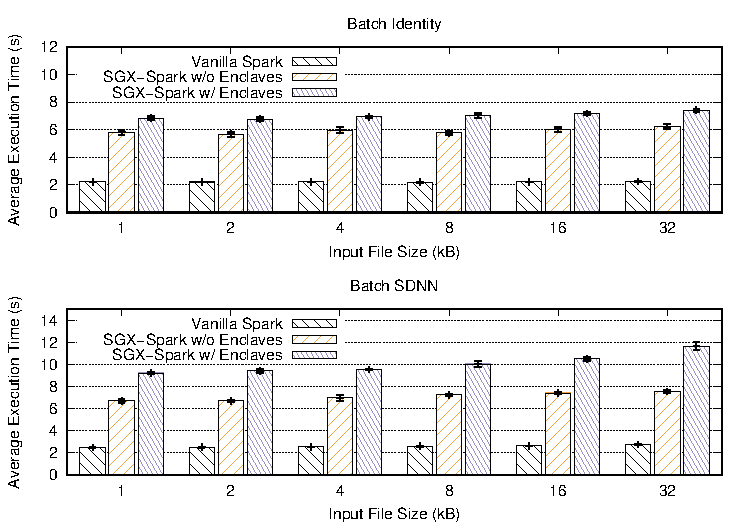
\includegraphics[width=.7\textwidth]{plots/input_size.pdf}
%    \end{figure}
%
%\end{frame}

\begin{frame}
    \frametitle{Evaluation \& Results}
    \framesubtitle{Results: Batch Execution - Big Load}

    \vspace{-15pt}

    \begin{figure}[T]
        \centering
        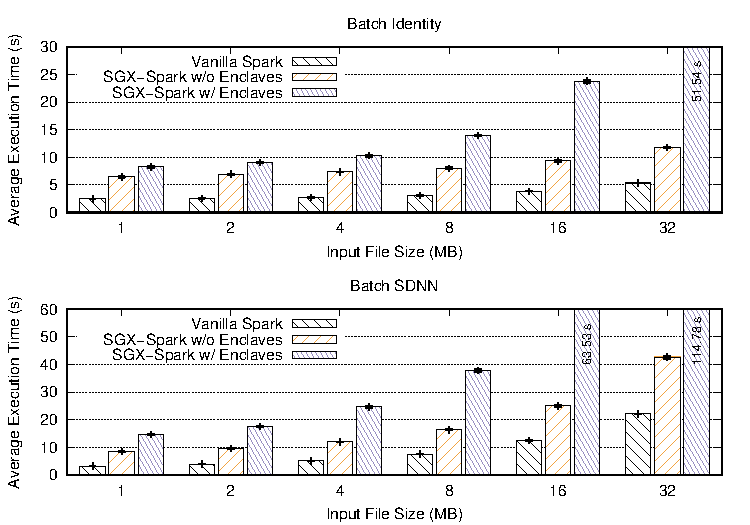
\includegraphics[width=.7\textwidth]{plots/big_input_size.pdf}
    \end{figure}

\end{frame}

%\begin{frame}
%    \frametitle{Evaluation \& Results}
%    \framesubtitle{Results: Stream Execution - Small Load}
%
%    \vspace{-15pt}
%
%    \begin{figure}[T]
%        \centering
%        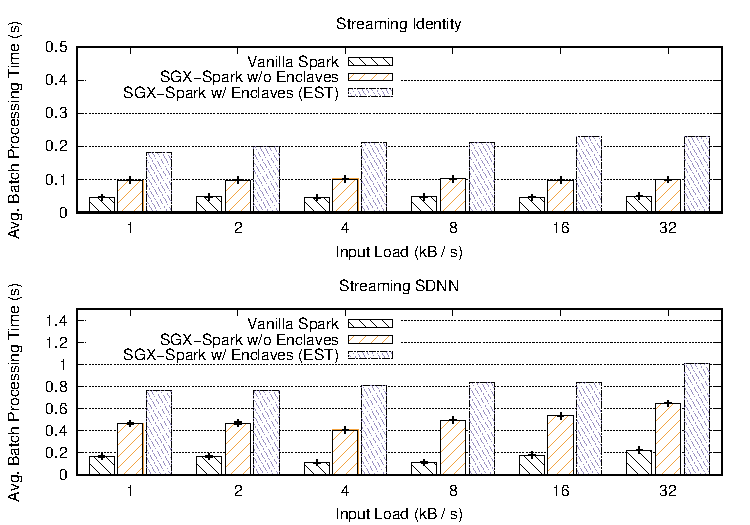
\includegraphics[width=.7\textwidth]{plots/throughput.pdf}
%    \end{figure}
%
%\end{frame}

\begin{frame}
    \frametitle{Evaluation \& Results}
    \framesubtitle{Results: Stream Execution - Big Load}

    \vspace{-15pt}

    \begin{figure}[T]
        \centering
        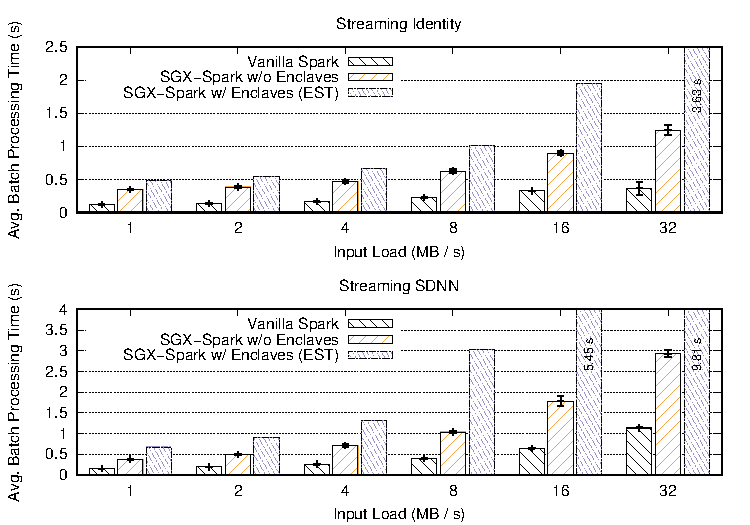
\includegraphics[width=.7\textwidth]{plots/big_throughput.pdf}
    \end{figure}

\end{frame}

\section{Conclusions and Further Work}
\label{sec:conclusions}
\sectionframe

\begin{frame}
    \frametitle{Summary}
    \framesubtitle{Critical Overview, Future Research, and Dissemination}

    \vspace{-20pt}

    \begin{itemize}
        \item Introduced a PoC of a \textbf{\textcolor{fgRed}{privacy-preserving streaming platform}}.
        \begin{itemize}
            \item Introduces $\times 4-5$ slowdown vs \textbf{vanilla Spark Streaming} (load $< 4$ MB per second).
            \item Requires \textbf{no changes} to the application source code.
            \item It is \textbf{reliable enough} to start trials in \textbf{\textcolor{fgRed}{production environments}}.
        \end{itemize}
        \item Proposed lines of research:
        \begin{itemize}
            \item Redo the experiments once the \textbf{final version} of SGX-Spark is released.
            \item Perform an economical evaluation of the cost of deploying our system to the cloud: \textbf{how expensive is privacy?}
            \item \textbf{Reduce the TCB} on the client side leveraging TEEs for low-power devices (\textit{e.g.} ARM TrustZone).
        \end{itemize}
        \item Further dissemination:
        \begin{itemize}
            \item Keynote session at DAIS'19 - Tuesday, June 18th (Copenhagen, DK).
            \item Poster session at the IEEE EMBC'19 - Thursday, July 25th (Berlin, GER).
        \end{itemize}
    \end{itemize}

\end{frame}

\section{Questions \& Observations}
\sectionframe

\end{document}
